\documentclass{article}[fleqn]

\usepackage{fancyhdr}
\usepackage{extramarks}
\usepackage{amsmath}
\usepackage{amsthm}
\usepackage{amsfonts}
\usepackage{tikz}
\usepackage[edges]{forest}
\usepackage[plain]{algorithm}
\usepackage{algpseudocode}
\usepackage[utf8]{inputenc} % Umlaute
\usepackage{ulem} % underline with wordwrap \uline
\usepackage{etoolbox}
\AtBeginEnvironment{align}{\setcounter{equation}{0}}
\usepackage{prooftrees} 
\usepackage{tikz}
\usepackage{tikz-qtree}
%\usetikzlibrary{graphdrawing.trees}
\usepackage{tabularx, caption}
\usepackage{ragged2e}
\usepackage{tcolorbox}
\usepackage{pifont}
\newcommand{\cmark}{\ding{51}}
\usepackage{subcaption}

\usetikzlibrary{automata,positioning}

% ///////////////////////
% Basic Document Settings
% ///////////////////////

\topmargin=-0.45in
\evensidemargin=0in
\oddsidemargin=0in
\textwidth=6.5in
\textheight=9.0in
\headsep=0.25in

\linespread{1.1}

% Tablestuff
\def\arraystretch{1.5}
\newcolumntype{L}{>{\RaggedRight} X}

\pagestyle{fancy}
\lhead{\hmwkAuthorName, \hmwkMatrikel}
\chead{\hmwkClass: \hmwkTitle}
\rhead{\firstxmark}
\lfoot{\lastxmark}
\cfoot{\thepage}

\renewcommand\headrulewidth{0.4pt}
\renewcommand\footrulewidth{0.4pt}

\newcommand{\splitter}{\noindent\rule{\textwidth}{1pt}}

\setlength{\parskip}{\baselineskip}%
\setlength\parindent{0pt}

% Tcolorbox
\definecolor{frame}{RGB}{214, 214, 239}
\definecolor{back}{RGB}{234, 234, 247}
\tcbset{colback=back,colframe=frame,coltitle=blue,boxrule=0mm,boxsep=6pt,left=2pt,right=2pt,top=0pt,bottom=0pt}

% ///////////////////////
% Create Problem Sections
% ///////////////////////

\newcommand{\enterProblemHeader}[1]{
    \nobreak\extramarks{}{Continuation on the next page\ldots}\nobreak{}
    \nobreak\extramarks{Exercise \arabic{#1} (Continuation)}{Continuation on the next page\ldots}\nobreak{}
}

\newcommand{\exitProblemHeader}[1]{
    \nobreak\extramarks{Exercise \arabic{#1} (Continuation)}{Continuation on the next page\ldots}\nobreak{}
    \stepcounter{#1}
    \nobreak\extramarks{Exercise \arabic{#1}}{}\nobreak{}
}



\setcounter{secnumdepth}{0}
\newcounter{partCounter}
\newcounter{homeworkProblemCounter}

% ///////////////////////////////////
% Initialize the problem counter here
% ///////////////////////////////////
\setcounter{homeworkProblemCounter}{1}
\nobreak\extramarks{Exercise \arabic{homeworkProblemCounter}}{}\nobreak{}

% ////////////////////////////
% Homework Problem Environment
% ////////////////////////////
% This environment takes an optional argument. When given, it will adjust the
% problem counter. This is useful for when the problems given for your
% assignment aren't sequential. See the last 3 problems of this template for an
% example.
%
\newenvironment{homeworkProblem}[1][-1]{
    \ifnum#1>0
        \setcounter{homeworkProblemCounter}{#1}
    \fi
    \section{Exercise \arabic{homeworkProblemCounter}}
    \setcounter{partCounter}{1}
    \enterProblemHeader{homeworkProblemCounter}
}{
    \exitProblemHeader{homeworkProblemCounter}
}

% ////////////////
% Homework Details
%   - Title
%   - Due date
%   - Class
%   - Section/Time
%   - Instructor
%   - Author
% ////////////////

\newcommand{\hmwkTitle}{Exercise 1}
\newcommand{\hmwkDueDate}{09.05.2019}
\newcommand{\hmwkClass}{EKI}
\newcommand{\hmwkClassTime}{}
\newcommand{\hmwkClassInstructor}{}
\newcommand{\hmwkAuthorName}{STUDENT NAME}
\newcommand{\hmwkMatrikel}{MAT NUMBER}

% //////////
% Title Page
% //////////

\title{
    \vspace{2in}
    \textmd{\textbf{\hmwkClass:\ \hmwkTitle}}\\
    \normalsize\vspace{0.1in}\small{\hmwkDueDate}\\
    \vspace{0.1in}\large{\textit{\hmwkClassInstructor\ \hmwkClassTime}}
    \vspace{3in}
}

\author{\textbf{\hmwkAuthorName, \hmwkMatrikel}}
\date{}

\renewcommand{\part}[1]{\textbf{
    \\[\baselineskip]
    \large Part
    \alph{partCounter}
    }\stepcounter{partCounter}}

% ///////////////////////
% Various Helper Commands
% ///////////////////////

% Useful for algorithms
\newcommand{\alg}[1]{\textsc{\bfseries \footnotesize #1}}

% For derivatives
\newcommand{\deriv}[1]{\frac{\mathrm{d}}{\mathrm{d}x} (#1)}

% For partial derivatives
\newcommand{\pderiv}[2]{\frac{\partial}{\partial #1} (#2)}

% Integral dx
\newcommand{\dx}{\mathrm{d}x}

% Alias for the Solution section header
\newcommand{\solution}{\textbf{\large \\Solution}}

% Probability commands: Expectation, Variance, Covariance, Bias
\newcommand{\calI}{{\cal I}}
\newcommand{\calM}{{\cal M}}
\newcommand{\eq}{\leftrightarrow}

\begin{document}

\maketitle
\pagebreak

% ///////////////////////
% Regular Problem example
% ///////////////////////
%\twocolumn
\begin{homeworkProblem}
    Describe the application types (PEAS) and the task environments of each of the following intelligent agents. Be sure to explain your reasoning and aussumptions.

    \begin{enumerate}
        \item Playing an online multiplayer game,
        \item Playing a game of Minesweeper,
        \item Robot vacuum cleaner.
    \end{enumerate}

    \solution{}

    \begin{table}[h]
        \setlength\extrarowheight{2pt}
        \begin{tabularx}{\textwidth}{|L||L|L|L|L|}
            \hline
            Agent Type & Perfomance Measure & Environment & Actuators & Sensors \\
            \hline \hline
            Online Multiplayer Game & 

            &

            &

            & 
            \\
            \hline
            Minesweeper &

            & 

            & 

            & 

            \\
            \hline
            Robot vacuum cleaner &

            &

            & 

            & 

            \\
            \hline 
        \end{tabularx}
        \caption{PEAS Exercise}
    \end{table}
\end{homeworkProblem}

\begin{homeworkProblem}
    Let $f(n) = c \cdot g(n) + d \cdot h(n)$ be an evaluation function, where $c$ and $d$ are constants.

    \begin{enumerate}
        \item Define $c, d, h(\cdot), g(\cdot)$ such that A* with this evaluation function acts as a breadth-first search.
        \item Define $c, d, h(\cdot), g(\cdot)$ such that A* with this evaluation function acts as a depth-first search.
        \item Define $c, d, h(\cdot), g(\cdot)$ such that A* with this evaluation function acts as a uniform cost search.
    \end{enumerate}

    You may assume that nodes contain all the information that we discussed in the lecture.

    \solution{}

\end{homeworkProblem}

\begin{homeworkProblem}
    Assume $h_a, h_b, h_c$ are admissible heuristics. Which of the following heuristics are admissible?
    \begin{enumerate}
        \item $h_1(n)=|h_a(n)-h_b(n)|$,
        \item $h_2(n)=2h_a(n)-(h_b(n)+h_c(n))$,
        \item $h_3(n)=\text{min } \{h_a(n)\cdot h_b(n),h_c(n)\}$
    \end{enumerate}

    \solution{}

        \begin{tcolorbox}[title=Definition]
            A heuristics $h$ is admissible, if for every node $n$ the following holds:
            \begin{enumerate}
                \item $h(n) \leq h^*(n) \text{ where } h^*(n)$ is the true cost from $n$ ($h$ is "optimistic");
                \item $h(n) \geq 0$;
                \item $h(g) = 0$ for every goal $g$ (follows from 1 and 2).
            \end{enumerate}
        \end{tcolorbox}

        \splitter

\end{homeworkProblem}

\begin{homeworkProblem}
    Prove that if the heuristics $h_1, \ldots , h_k$ are all monotone (consistent), then
    \[h(n) = \text{max } \{h_1(n), \ldots , h_k(n)\}\]
    is admissible. Is $h$ also consistent?

    \solution{}

\end{homeworkProblem}

\newpage

\begin{homeworkProblem}
    Driving from your home at node $A$ to university at node $G$, you usually take the shortest path $A \to E \to D \to G$. Due to recently started construction work, however, the segment $E \to D$ would take you a bit longer than usual to cross.

    Use the A* algorithm using the given heuristic function $h$ on the city graph below in order to see if there is a shorter path from $A$ to $G$. In which order are the nodes expanded? Show the contents of the priority queue at iteration. If multiple nodes have the same priority, expand the one that comes first alphabetically.

    \begin{figure}[h]
        \centering
        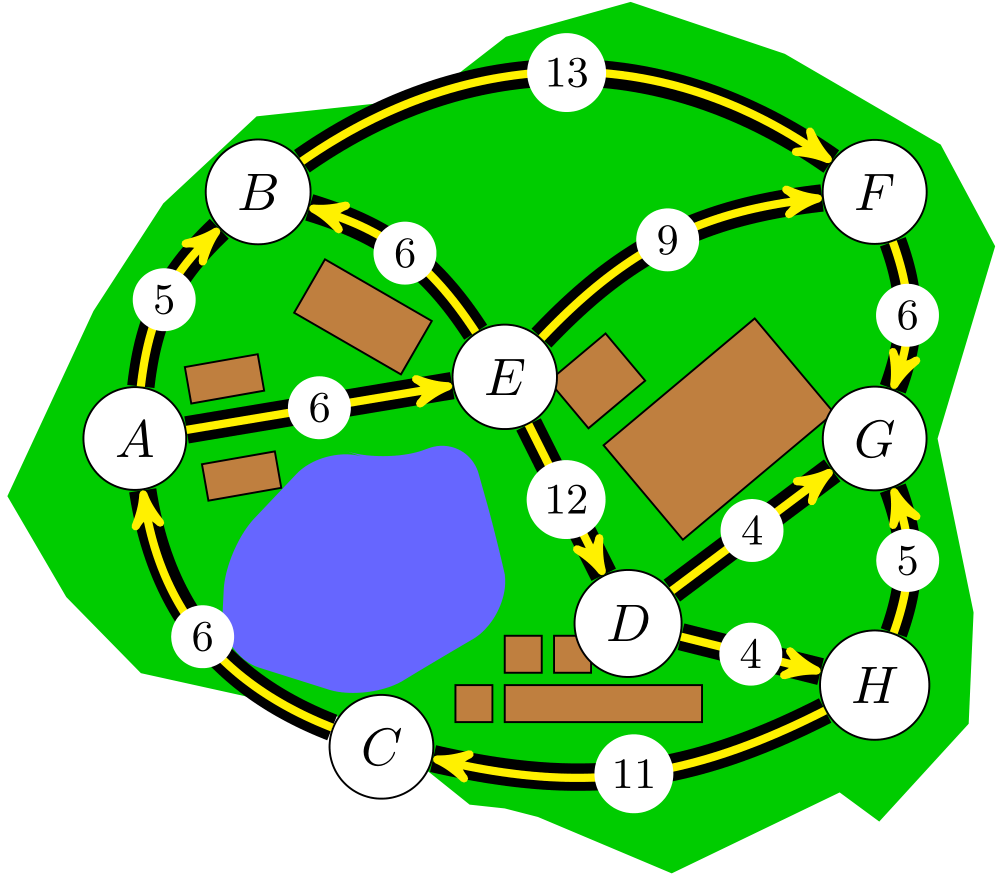
\includegraphics[scale=0.5]{citygraph.png}
    \end{figure}

    \[h(A)=12, h(B)=11, h(C)=10, h(D)=3, h(E)=6, h(F)=6, h(G)=0, h(H)=4\]

    \solution{}

\end{homeworkProblem}

\newpage

\begin{homeworkProblem}
    Consider the following graph (the gray nodes are goal nodes):

    \begin{figure}[h]
        \centering
        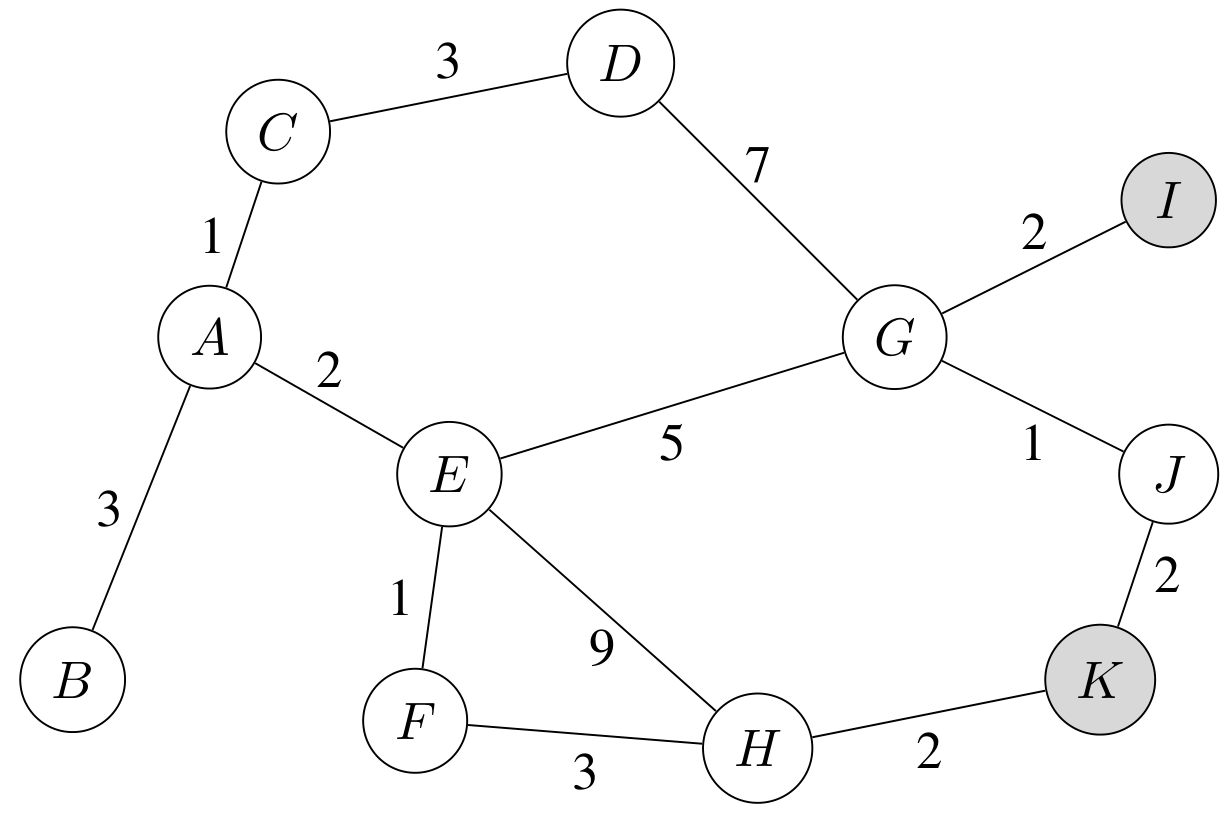
\includegraphics[scale=0.5]{graph.png}
    \end{figure}

    Use the listed search strategies on the given graph to look for a goal node, starting from the node $A$ (depth 0). In case you can expand several nodes and the search strategy does not specify the order, choose the noes in alphabeetic order. Where applicable, specify the contents of the \textit{frontier} and the \textit{explored set} for each step or the contents of the call stack for recursive approaches.

    \begin{itemize}
        \item Breadth-first search with goal test at generation time,
        \item Uniform cost search.
        \item Depth-first search with goal test at expansion time, iterative,
        \item Depth-limited search (use a limit of 2),
        \item Iterative deepening search.
    \end{itemize}

    \solution{}

\end{homeworkProblem}

\begin{homeworkProblem}
    consider again the 8-Puzzle discussed in the lecture. Consider the discussed heuristics
    \begin{itemize}
        \item $h_1(n)$: number of misplaced tiles,
        \item $h_2(n)$: Manhattan distance.
    \end{itemize}

    Show whether the two suggested heuristics are admissable and/or consistent (monotonic).

    \solution{}
\end{homeworkProblem}

\begin{homeworkProblem}
    Decide and explain which of the following statements are true and which are false? Back up your answer with proofs or counterexamples.

    \begin{enumerate}
        \item Breadth-first search always expands at least as many nodes as an A* search with an admissable heuristic.
        \item The A* algorithm yields an optimal path in a graph search if the used heuristic is admissable.
        \item Every admissable heuristic is also consistent.
    \end{enumerate}

    \solution{}

\end{homeworkProblem}
\end{document}
